%%%% Various options for document class.
%%\documentclass[usenatbib, a4paper, 11pt]{aastex}
%%\documentclass[preprint, 11pt, a4paper]{aastex}
%%\documentclass[twocolum]{revtex4}
%%\documentclass{report}
\documentclass[useAMS,usenatbib]{mn2e_x}

%\usepackage{psfig,morefloats,url}
%use preprint2 for 2 columns paper.

%% declare any packages used
\usepackage{graphicx}
\usepackage{natbib}
\usepackage{graphicx}
\usepackage{color}
\usepackage{pdfpages}
\usepackage{appendix}
\usepackage{subfigure}
%\usepackage{epsfig}
%\usepackage[dvips]{color}
%\usepackage{aabib}


%\marginparwidth = 25pt
\citestyle{aa}
\addtolength{\topmargin}{-.5in}
%\addtolength{\bottommargin}{-1in}
%% This command added as margins are wrong in mn2e, it appears. 
%% Not needed for other classes
\usepackage{float}



%%%%%%%%%%%%%%%%%%%%%%%%%%%%%%%%%%%%%%

\begin{document}
%% define bibstyle and other definitions
\bibliographystyle{aabib}
%% renew commands
%%\renewcommand{\labelitemi}{$.$}

%% Codes
\def\py{\textsc{Python} }
\def\tar{\textsc{Tardis} }
\def\cld{\textsc{Cloudy} }
\def\agn{\textsc{Agnspec} }


%% Lines and ions
\def\civ{C~\textsc{iv}}
\def\nv{N~\textsc{v}}
\def\heii{He~\textsc{ii}}
\def\ovi{O~\textsc{vi}}
\def\la{Ly$\alpha$}
\def\ha{H$\alpha$}

%% Journal definitions
\def\araa{ARAA}
\def\nat{Nature}
\def\apjl{ApJ Letters}
\def\aapr{AAPR}
\def\ssr{SSR}
\def\apj{ApJ}
\def\pasp{PASP}
\def\aap{A\&A}
\def\mnras{MNRAS}
\def\aj{AJ}
\def\rmxaa{RMXAA}

%%%%%%%%%%%%%%%%%%%%%%%%%%%%%%%%%%%%%%
%
%          TITLE AND AUTHORS
%
%%%%%%%%%%%%%%%%%%%%%%%%%%%%%%%%%%%%%%%

\title
{
The effect of clumpy outflows
and disk anisotropy on quasar unification scenarios
}


% [Matthews, J.]
% \author[Matthews, J.]{James Matthews \\
% {\sl  Supervisor: Prof. Christian Knigge} \\
% {\sl School of Physics \& Astronomy, University of Southampton,
%   Southampton, SO17 1BJ, UK}}

\author[Matthews et al.]{J.~H.~Matthews$^1$\thanks{jm8g08@soton.ac.uk}, C.~Knigge,$^1$
N.~Higginbottom,$^1$ K.~S.~Long,$^2$ S.~A.~Sim,$^3$ and S.~W.~Mangham
\medskip  
\\$^1$School of Physics and Astronomy, University of Southampton, Highfield, Southampton, SO17 1BJ, United Kingdom
\\$^2$Space Telescope Science Institute, 3700 San Martin Drive, Baltimore, MD, 21218
\\$^3$School of Mathematics and Physics, Queens University Belfast, University Road, Belfast, BT7 1NN, Northern Ireland, UK}

\date{\today}
%\\
%Supervisor: Prof. Christian Knigge\\
%{\sl School of Physics \& Astronomy, University of Southampton,
%  Southampton, SO17 1BJ, UK}}


%%%%%%%%%%%%%%%%%%%%%%%%%%%%%%%%%%%%%%
%
%          ABSTRACT
%
%%%%%%%%%%%%%%%%%%%%%%%%%%%%%%%%%%%%%%%

\maketitle


\begin{abstract} 
% Broad absorption lines (BALs) in the ultraviolet 
% are seen in $\sim20\%$ of quasi-stellar objects (QSOs). 
% Blue-shifted broad absorption lines (BALs) are the most direct evidence of 
% accretion disk `winds' in such systems; mass loaded outflows
% emanating from the disk that may be driven by line forces or
% magnetic processes. 
Various unification schemes for
QSOs and active galactic nuclei (AGN) have proposed
that the broad emission line region is roughly cospatial
with broad absorption line (BAL) gas and much of the phenomenonology of AGN
can be explained by a simple geometrical picture involving an accretion
disk and associated outflow. Here, we test this paradigm by 
utilising our state-of-the-art radiative transfer code to produce synthetic spectra
from simple biconical disk wind models. In particular, we expand on our previous 
work in which a benchmark model for BAL quasars was produced. 
We find that a simple treatment of clumping (`microclumping') 
allows for a more realistic X-ray luminosity in the model by lowering the 
ionization parameter. We examine the X-ray properties of this new model
and find good agreement with existing X-ray samples of AGN and QSOs.
We find that clumping enhances the H recombination and collisionally excited resonance lines,
causing strong line emission (???EW) to emerge at the low inclination angles, 
which represent quasars within this unification scenario.
We also treat Hydrogen using a `macro-atom' approach in order to 
examine the effect of recombination on Hydrogen emission lines, and
this results in significant line emission in Lyman~$\alpha$ and the Balmer series.
However, we are unable to produce line emission with comparable equivalent widths
to existing quasar composites, due to a fundamental constraint arising
from the anisotropy of emission from a classical thin disk. We briefly 
explore the effect of relativistic beaming, gravitational redshift and 
light bending on the angular distribution of disk continuum emission. 
We find that these general relativistic effects do cause the disk to
emit more isotropically, but this is not yet sufficient to produce a
self-consistent model. We discuss a number of potential solutions. 
Overall, our work suggests that geometric unification
involving an ADW is a promising scenario, but our results 
pose a number of difficult challenges to such a model.
Determining the true geometry of ADWs and uncovering the true disk spectral 
(and angular) energy distribution are key next steps if we are to build up a 
holistic picture of the Quasar population.
\end{abstract}

%\begin{keywords}
%AGN: outflows
%\end{keywords}



%%%%%%%%%%%%%%%%%%%%%%%%%%%%%%%%%%%%%%
%
%          INTRODUCTION
%
%%%%%%%%%%%%%%%%%%%%%%%%%%%%%%%%%%%%%%%
\section{Introduction}

Introduction focussing on key points

\begin{itemize}
\item standard wind + BALQSO introduction
\item focus on unification and that we are testing it
\item some discussion of scales, referencing e.g. reverb maps, variability, microlensing, Arav 
\item clumping background: stellar winds, clumping in AGN winds, variability
\end{itemize}
%%\item 

% Outflows are ubiquitous in active galactic nuclei (AGN) and quasi-stellar objects (QSOs).
% They can take the form of highly collimated radio jets \citep{bellonijet2010}, 
% or mass-loaded `winds' emanating from the accretion disk. 
Approximately $20\%$ of QSOs exhibit broad absorption lines (BALs) in the ultraviolet,
providing clear evidence for outflowing absorbing material
\citep{weymann1991, knigge2008, turnermiller2009,allen2011}.
The simplest explanation for the incidence of 
BALs in quasar samples is in terms of an accretion disk wind (ADW). 
In this paradigm, the BALQSO fraction is associated with
the covering factor of the outflow.
Indeed, many have gone further, and suggested that the diverse phenemonology
of luminous AGN and QSOs can be broadly explained by
into a simple picture of geometric unification \citep[e.g.]{MCGV95, elvis2000}. 
In such a model, a biconical wind rises from 
a thin accretion disk \cite{shakurasunyaev1973}, approaching velocities
close to $\sim0.1c$. Depending on viewing angle, an observer 
may then see a BALQSO, LoBAL-QSO or normal `Type 1' quasar- with 
broad emission lines superposed on a disk-like continuum. 

The UV spectrum of {\em non-BAL} QSOs is typified by a series
of strong emission lines (e.g. \la, \civ, \nv) with an underlying blue continuum
- the so-called {\sl `big blue bump'} (BBB). The BBB is normally attributed to blackbody-like
emission from an accretion disk surrounding the central black hole (REF), similar
to that described by \cite{shakurasunyaev1973}. However,
a number of issues have arisen relating to this model. First, 
AGN/QSO spectra exhibit a `break' in the spectrum at around $1000$~\AA 
which scales only weakly with black hole mass. This potentially 
suggests a problem with a thin disk model (e.g. Antonucci). 
However, it is possible that this is the result of incorrect intergalactic medium
(IGM) corrections (REF) or corresponds to the temperature 
at which a line-driven wind carries mass away from the system (laor davis).
Second, results from microlensing (REFs) imply that the disk emission 
region is $\sim4$ times larger than one might expect from a Shakura-Sunyaev
model. Inhomogenous disks have been proposed as an alternative (REFs).
These observations appear to pose problems for the thin disk model of luminous,
sub-Eddington AGN. However, recent results from \cite{capellupo2015} find 
that if one includes a combination of mass-loss, general relativity (GR) and Comptonisation
then AGN SEDs can, in general, be fitted well with accretion disk models.
Uncovering the intrinsic disk SED and understanding the effect of the outflow on the accretion 
mechanism is clearly crucial if we are to properly understand the physical nature
of AGN.

The geometry and size of the BLR is also a matter of contention. 
The main constraints on the emission region size come from microlensing (REFs)
and reverberation mapping (REFs). While these observations have mostly been
carried out for Seyfert galaxies, there are also a few instances of these methods
being applied to quasars (REFs). A number of different proposals have been made 
for the origin of the BLR. Early AGN unification scenarios posited that the broad emission lines
where produced by clouds of plasma orbiting fairly close to the BH (refs).
Since then, multiple interpretations of a disk wind model have been proposed,
with varying radii and geometries (refs). 

In this paper, we attempt to test the disk wind paradigm 
using Monte Carlo radiative transfer and photoionization calculations.
In section 2, we describe our code. In section 3, we briefly discuss some 
of the successes and failures of our previous benchmark model for BALQSOs 
\citep[][hereafter H13]{higginbottom2013} and outline the model, including 
a description of our clumping prescription. In section 4, we present the results 
from a clumped model which successfully reproduces
the observed ionization state while maintaing realistic X-ray properties.
In section 5 we discuss our results, focussing particular on the anisotropy of 
disk emission and GR effects, and finally, in section 6, we summarise our findings.



%  a simple model in which
% quasars are unified by BH mass, Eddington ratio and viewing angle can successfully
% reproduce UV, optical and X-ray properties of {\em both} 
% BALQSO's and normal emission line quasars. 

% Geometrical unification pictures have suggested that 
% the BAL fraction can be interpreted as the covering factor
% of an accretion disk wind (refs), and some also propose
% that this disk wind may also be the source of the broad emission
% lines (BELs) seen in QSOs (refs). 
% Alternatively, there are a number of evolutionary models in which
% QSOs spend approximately $20\%$ of their lifetime as BALQSOs in which the outflow
% has a high covering factor (refs). 
% It is also possible that BALQSOs lie in a distinct region
% in terms of Eddington ratio (refs), but this is somewhat refuted 
% by observations (refs). % to e.g. Allen and Eigenvector I papers Ledd of BALQSOs
% Orientation, evolution, black hole mass and eddington ratio 
% may all have an effect on the BAL fraction (refs),  % to e.g. Allen
% and the importance of each must be understood to build up coherent picture.


% The driving mechanism for accretion disk winds is uncertain. The winds responsible 
% for BALs must at least have some line-driven component,
% as very strong resonance lines exert a strong line force on the 
% gas (refs). Line-driven winds are notoriously unstable (refs),
% meaning that one may expect an unstable and inhomogenous 
% velocity and density structure (refs). Magnetically driven
% winds may also produce clumpy winds or `clouds' of material which
% are magnetically confined (refs here to Shlosman, Begelman and the like).
% Describe mechanism.

% Evidence for an inhomogenous density structure in an accretion disk wind 
% and/or the broad emission line region comes from multiple sources. 
% Microlensing observations of absorption troughs suggest that different lines of sight 
% exhibit varying velocity components (refs), and BALQSO troughs 
% are known to exhibit variability (refs).

% trend of L_X with radio jets and Sy 1s
% trend of BALs with radio loudness
% see MCGV95




\section{Method: Ionization and Radiative Transfer}

We use a code Python described extensively by LK02, S05, H13, M15...

\subsection{Ionization Scheme}

We adopt the same hybrid scheme described by \cite{M15}...
% , but we have improved our ionization scheme
% for simple ions to explicitly solve the rate equations based on MC estimators.

\subsection{Macro-atoms}


\section{A Simple Biconical Disk Wind Model for QSOs}

\begin{figure}
\centering
\includegraphics[width=0.45\textwidth]{figures/fig2_cartoon.png}
\caption
{
A cartoon showing the geometry and some key parameters of
our biconical wind model.
}
\label{fig:alpha_ox}
\end{figure}

\subsection{A Benchmark Model for BALQSOs}

\cite{higginbottom2013} presented a benchmark model for
(BAL)QSOs...introduce key parameters. 
% which successfully reproduced BAL features 
% in synthetic spectra using \py. However, the model
% had a few key drawbacks when considering its potential
% for unification. First, it failed to produce significant
% broad emission lines at non-BAL viewing angles; this is 
% a key requirement for a unified QSO model. Second,
% the model was significantly X-ray weak, as it was found
% that an X-ray luminosity comparable to that of a QSO 
% over-ionized the wind, resulting in no UV resonance 
% line absorption features.

% \begin{table}
% \begin{tabular}{p{3cm}p{4cm}}
% \hline Free Parameters 	&	 Value \\ 
% \hline \hline 
% $M_{BH}$ 	 &	 $1\times 10^9~\rm{M_{\odot}}$ \\ 
% $\dot{M}_{acc}$ 	 &	 $5~M_{\odot}yr^{-1} \simeq 0.2~\dot{M}_{Edd}$\\ 
% $\alpha_X$ 	 &	 $-0.9$ \\ 
% $L_{X} $ 	 &	 $1\times10^{43}~\rm{ergs~s^{-1}}$\\ 
% $r_{disk}(min)=r_{X}$   &	 $6r_g=8.8\times10^{14}~{\rm cm}$ \\ 
% $r_{disk}(max)$   &	 $3400r_g = 5\times10^{17}~{\rm cm}$ \\ 
% $\dot{M}_{wind}$  &	 $5~M_{\odot}yr^{-1}$ \\ 
% $r_{min}$ 	&	 $300r_{g} = 4.4\times10^{16}~{\rm cm}$\\ 
% $r_{max}$ 	&	 $600r_{g} = 8.8\times10^{16}~{\rm cm}$ \\ 
% $\theta_{min}$ 	&	 $70.0^{\circ}$ \\ 
% $\theta_{max}$ 	&	 $82.0^{\circ}$ \\ 
% $\lambda$ 	&	 $0$ \\ 
% $v_{\infty}$ 	&	 $v_{esc}$(f=1) \\ 
% $R_v$ 	        &	 $1\times10^{18}$cm \\ 
% $\alpha$ 	&	 $1.0$ \\
% \hline 
% Derived Parameters 	&	 Value \\ 
% \hline \hline
% $L_{\nu}(2500\mbox{\scriptsize{\AA}})$&	 $6.3\times10^{30}~\rm{ergs~s^{-1}~Hz^{-1}}$\\ 
% $L_{\nu}(2keV)$   &	 $1.2\times10^{25}~\rm{ergs~s^{-1}~Hz^{-1}}$\\ 
% $L_{bol}$ 	 &	 $2.4\times10^{46}~\rm{ergs~s^{-1}}$\\
% $M_{bol}$ 	 &	 -27.4\\ 
% $M_u$            &	 -26.2\\ 
%  $\alpha_{OX} $ 	 &	 -2.2\\ 
% \end{tabular}
% \caption{Wind geometry parameters used in the benchmark model.}
% \label{wind_param}
% \end{table}

\subsection{Potential for unification}

\subsection{Clumping}



To take account of clumping in our outflow we adopt a simple parameterization
used in stellar wind modelling, known as {\em microclumping}. 
The key assumption here is that typical clump sizes
are much smaller than the typical photon mean free path, and thus the clumps are 
both geometrically and optically thin. This approach is typically 
known as microclumping and allows one to introduce a `filling factor', $f$, which is the 
fraction of the volume of the plasma filled by clumps. We can then introduce the 
density enhancement, $D$, which is simply 

\begin{equation}
D = \frac{1}{f}
\end{equation}

One can then multiply all densities in the model by $D$, and all emitting volumes
by $f$, meaning that all $\rho^2$ processes 
(such as collisional excitation and recombination) will be enhanced, 
while opacities remain unchanged (for fixed ionization state). A factor $f$ is also
applied to the opacities such that opacities which scale only with $\rho$ are not
increased. Clumping the wind has an important effect on the ionization state and has
been proposed as a solution to the so-called `over-ionization problem' in 
disk winds (refs). This is the main motivation for incorporating microclumping
into our model.  


\section{Results}

\subsection{Physical Conditions and Ionization State}

Show that clumping stops over-ionization.

\subsection{Synthetic Spectra}

Present a spectrum of the UV and possible optical too.

\subsection{X-ray Properties}

discuss the figure showing X-ray properties briefly. 
Present an X-ray spectrum? compare to observations e.g. Giustini?

\begin{figure*}
\centering
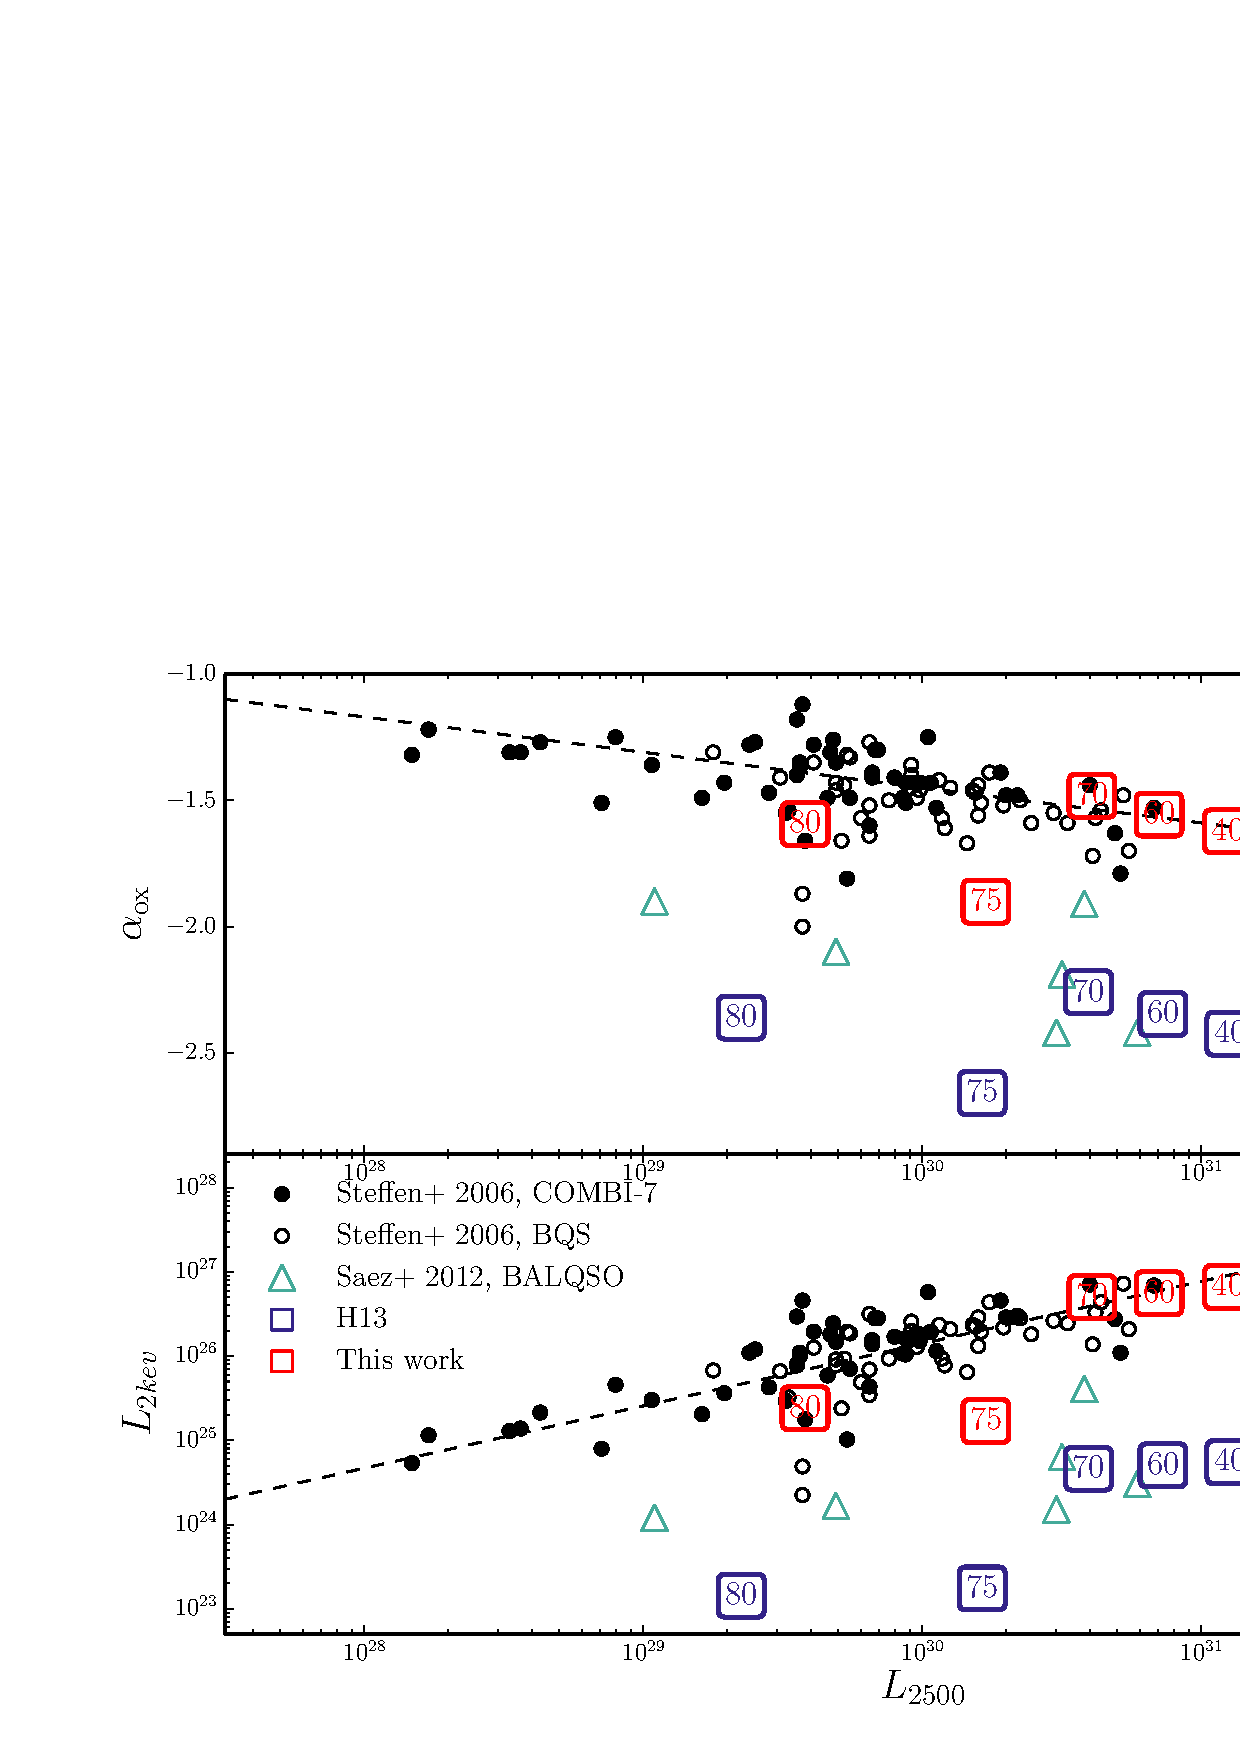
\includegraphics[width=1.0\textwidth]{figures/alpha_ox_both.png}
\caption
{
X-ray properties of the H13 and clumped model (text filled 
squares), plotted against monochromatic luminosity 
at 2500\AA. Also plotted are the samples considered by
Saez et al. 2012 on a similar plot; The COMBI-7 AGN sample (ref),
the BQS sample (ref) and the Saez et al. (2012) sample of BALQSOs.
}
\label{fig:alpha_ox}
\end{figure*}


\section{Discussion}

\subsection{Anisotropy of disk emission}

Discuss the importance of the angular distribution of the disk SED on line
(limb-darkened, foreshortened, etc.)

\subsection{General relativistic effects}

Can GR effects offer a potential solution? (not quite!)

\subsection{Wind reprocessing}

How would wind reprocessing help?

\subsection{The BALQSO fraction and wind covering factor}

A brief comment, citing Goodrich / Krolik \& Voit on the 
way in which anisotropy / attenuation affect the inferred
BAL fraction. We also need to be aware that there will be a number of selection
effects in building up the composites, and we should discuss these
and the subtleties involved. 

\begin{figure}
\centering
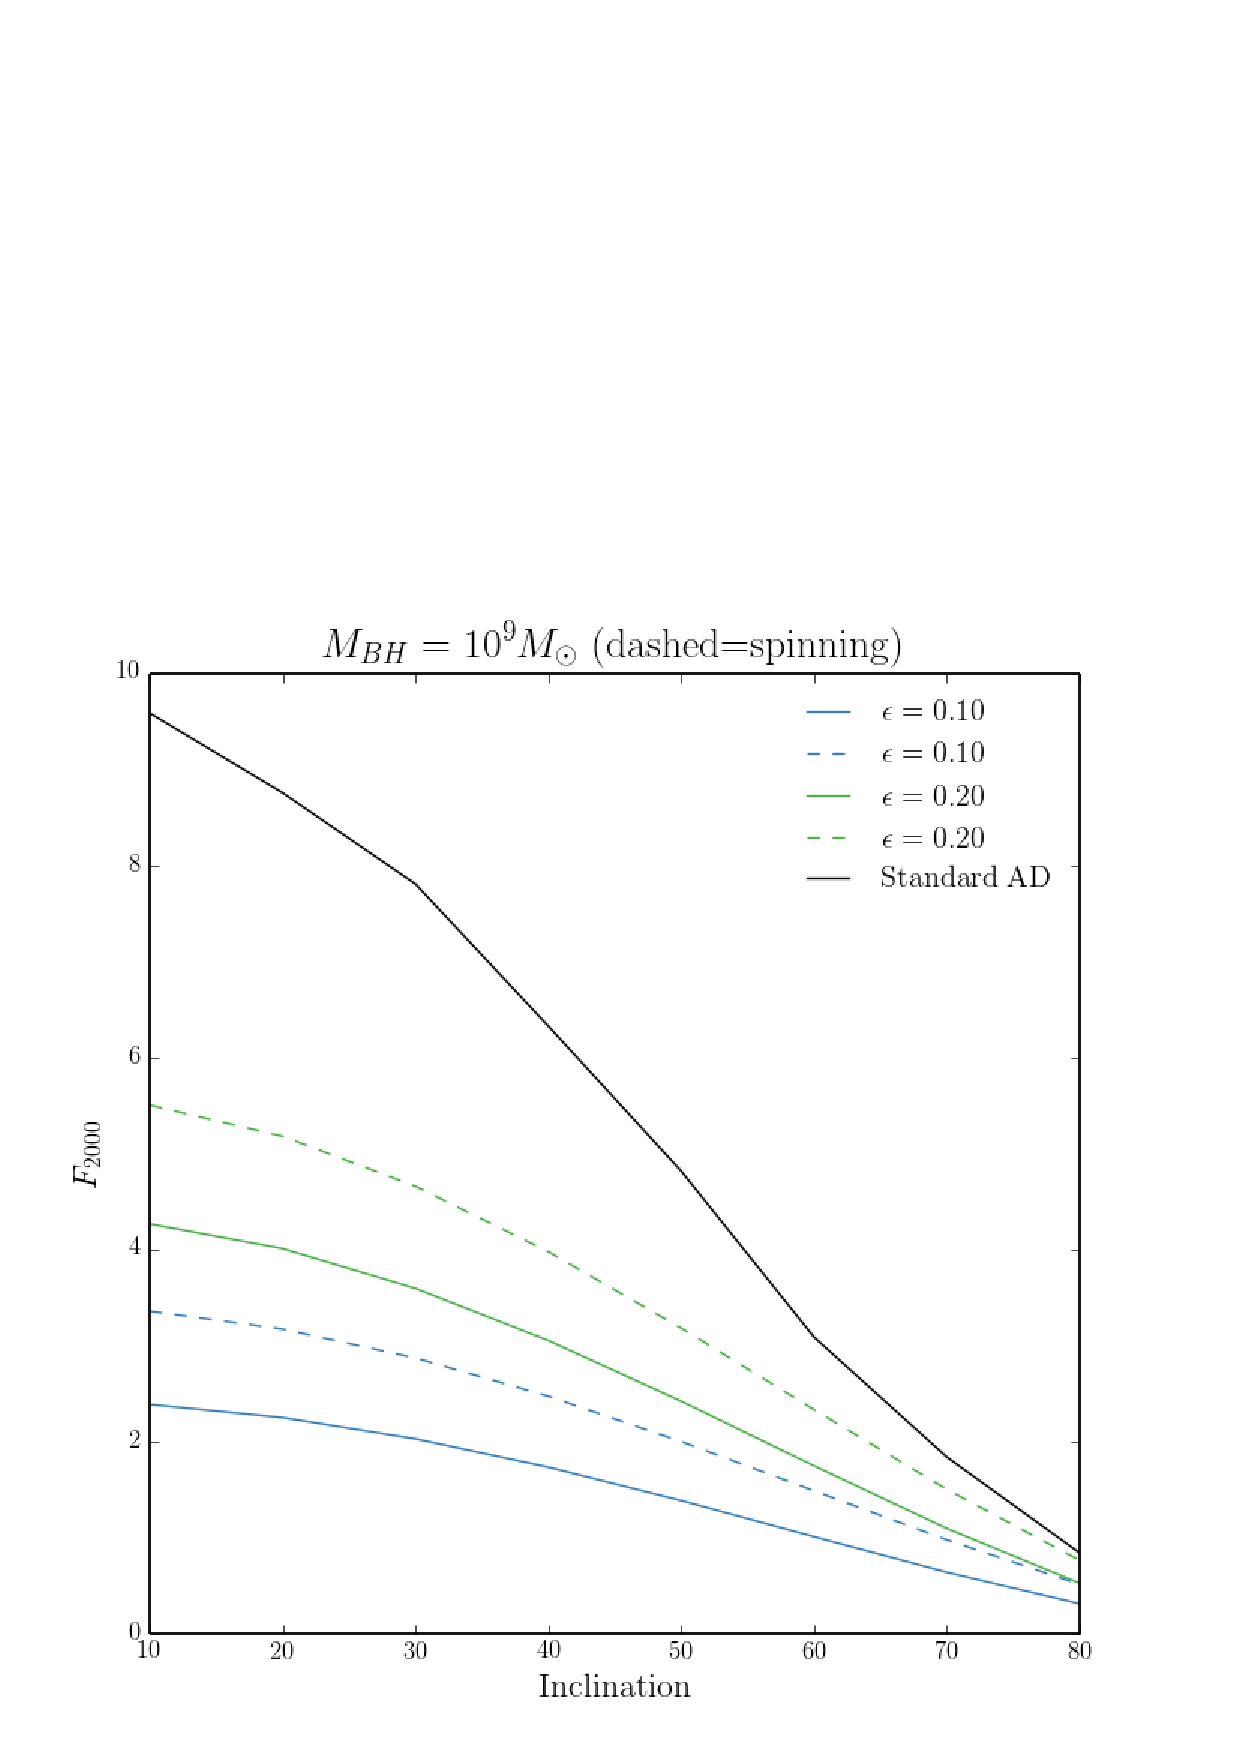
\includegraphics[width=0.45\textwidth]{figures/f2000_m9.png}
\caption
{
$F_\lambda$ at $2000$~\AA\ as a function of inclination from
\agn\ models. Spectra are computed for BH of $10^9~M_\odot$ with
a number of different BH spins and Eddington fractions. The black line
shows a standard multi-temperature blackbody AD model.
}
\label{fig:alpha_ox}
\end{figure}




\section{Summary}

Main points:

\begin{enumerate}
\item We have introduced a simple, first-order treatment 
of clumping in our model, and found that it can now maintain
the required ionization state while agreeing well with the X-ray
properties of AGN/QSOs.
\item We find that clumping also causes a significant 
increase in the strength of the  emission
lines produced by the model. This is true both
of collisionally excited resonance lines (such as \civ, \nv)
and recombination lines (such as \la, \ha\ and the Balmer series).
\item The line EWs in our models are not comparable to those in Quasar composite
spectra. This is due to a fundamental constraint discussed in section ?. If the BLR
emits fairly isotropically then for an anisotropic classical thin accretion disk
it is not possible to achieve line ratios at low inclinations that are comparable to
those at high inclinations. This is a robust conclusion which 
is independent of the assumed BLR geometry. 
\item We have examined the effect of GR on our disk SED, using the disk atmosphere
and GR ray-tracing code AGNSPEC. While including GR effects
does cause the disk SED to become significantly more isotropic,
the effect is not large enough to produce uniform line to continuum ratios
with viewing angle. We discuss other solutions to this problem in section ?; 
It is possible that a combination of GR and reprocessing by the wind could provide a 
solution, and a number of complicated selection effects may be at work
in the building of the quasar composites. Nevertheless,
our conclusions pose a challenge to the current unification picture.
\end{enumerate}


\section*{Acknowledgements}

%% \texttt{mn2e.cls} \textsc{Latex} document class. 


\bibliography{mybib.bib}
\newpage
%\appendix
\end{document}
